\documentclass[12pt,openright,twoside]{report}
\usepackage[portuguese]{babel}

\title{\textbf{Laboratórios de Informática: \\2ºDocumento em Português}}
\author{João Pedro Nunes Vieira \\NºMec.:50458 \\MIECT}
\date{\today}
\usepackage{graphicx}

\begin{document}
\graphicspath{ {/home/jp/Desktop/LI/Imagens} }
\tableofcontents
\renewcommand{\partname}{Parte}
\renewcommand{\chaptername}{Tema}
\renewcommand{\contentsname}{Índice}

\chapter{TESTE}

\section{Verificação de translineação:}
OLá\LaTeX!, vamos testar a ver se isto faz translineação, bora lá. Necessidade. Boa!
\\
\subsection{Tamanhos de texto:}
Posso {\small mudar} de {\huge tamanho} de letra sempre que me apetecer. Essa \Large mudança permanece em efeito{\normalsize até} ao próximo comando de mudança de tamanho,caso exista,\normalsize\space ou até ao fim do bloco(delimitado por \{ e\}) onde está inserida.
\subsubsection{Listas e Enumerações:}
Texto de exemplo.

\begin{itemize}
\item este é um item;
\item[+] este é outro item;
\item[UA -] ultimo item.
\end{itemize}

\renewcommand{\theenumi}{\Roman{enumi}}
\begin{enumerate}
\item Item em numeração Romana;
	\renewcommand{\theenumi}{\alpha{enumi}}
	\begin{enumerate}
	\item Este é um item em alpha num;
	\item Este é outro item em alpha num;
	\item Ultimo item alpha num. 
	\end{enumerate}
\renewcommand{\theenumi}{\Roman{enumi}}
\item este é outro item;
\item ultimo item.
\end{enumerate}

\subsubsection{Figuras e Gráficos:}

\begin{figure}[h] %h - posição auto; t - topo da pag; b - fundo da pag; p - isolado numa pagina
\centerline{\fbox{/home/jp/DEsktop/LI/Imagens}} %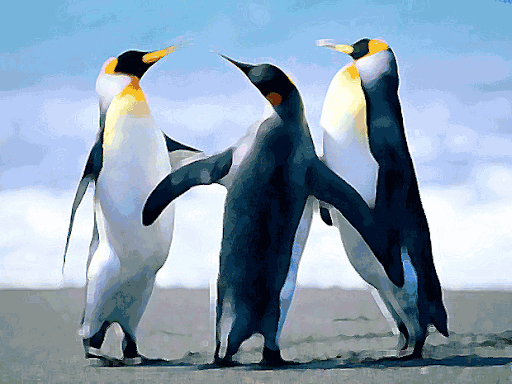
\includegraphics[scale=1.5]{pinguins}??
\caption{Legenda da figura}
\end{figure}

\begin{table}[htp]
\caption{Exemplo de uma tabela}
\centerline{Conteúdo de uma tabela}
\label{tabela-exemplo}
\end{table}



\end{document}